\documentclass[professionalfonts, aspectratio=169]{beamer}  
\usefonttheme{serif}                                        % Font theme: serif
\usepackage[utf8]{inputenc}                                 % Allows the use of different input encodings
\usepackage{graphicx}                                       % Enhanced support for graphics
\usepackage{amsmath}                                        % Enhances the typesetting of mathematics
\usepackage{amsfonts}                                       % Extra mathematical fonts
\usepackage{amssymb}                                        % Extra mathematical symbols
\usepackage{threeparttable}                 % For table notes
\usepackage{tikz}
\usetikzlibrary{shapes,arrows,positioning}
\usepackage{booktabs}                                       % Enhances the quality of tables
\usepackage{pgfplots}
\pgfplotsset{compat=1.17}
\usepackage{multirow}
% link settings
\usepackage{hyperref}                       % For hyperlinks
\usepackage[authoryear]{natbib}             % For bibliography

\usepackage{appendixnumberbeamer} % Numbering appendixes in beamer
\pdfstringdefDisableCommands{
  \def\translate{}
}
\usepackage{dcolumn}
\setbeamertemplate{navigation symbols}{} % Remove navigation symbols
\setbeamertemplate{footline}[frame number] % Add page number

% \setbeamercovered{transparent}  % Semi-transparent overlay

%---- Set the title page ----%
\title{Risk Adjustment, Self-Selection and Plan Design \\ in Medicare Advantage}
\institute{Stony Brook University}
\author{Zhu Liang}
\date{\today}

%---- Begin the document ----%
\begin{document}

\AtBeginSection[] % At the beginning of each section...
{
  \begin{frame}[noframenumbering, plain] % Create a new frame without a frame number
    \tableofcontents[currentsection] % Display the table of contents for the current section
  \end{frame}
}

\begin{frame}[noframenumbering, plain] % title frame without a frame number
    \titlepage
\end{frame}

%---- The slides structure ----%
\section{Background}
\begin{frame}{Medicare Market}
% insert the picture from figures/images/medicare_market.tex and center it
\begin{figure}
  \centering
  \resizebox{0.6\textwidth}{!}{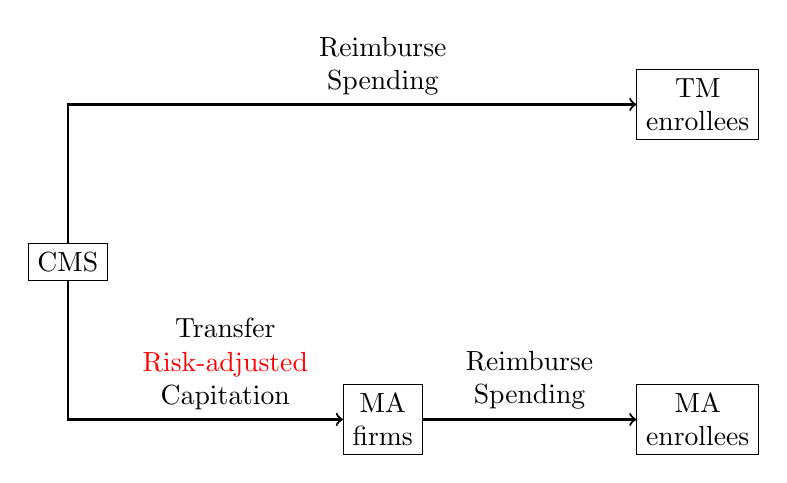
\begin{tikzpicture}
    \node[draw] (CMS) at (0,2) {CMS};
    \node[draw, align=center] (TM) at (8,4) {TM \\ enrollees};
    \node[draw, align=center] (MA) at (8,0) {MA \\ enrollees};
    \node[draw, align=center] (MAf) at (4,0) {MA \\ firms};

    \draw[->, thick] (CMS.north) |- (TM.west);
    \draw[->, thick] (CMS.south) |- (MAf.west);
    \draw[->, thick] (MAf.east) -- (MA.west) node[midway, above, align=center] {Reimburse \\ Spending};

    \node[above, align=center] at (4,4) {Reimburse \\ Spending};
    \node[above, align=center] at (2,0) {Transfer \\ \textcolor{red}{Risk-adjusted} \\ Capitation};
\end{tikzpicture}}
\end{figure}

CMS allows
\begin{itemize}\small
  \item Medicare Advantage (MA) firms to design plans,
  \item Consumers to choose between Traditional Medicare (TM) or MA plans.
\end{itemize}
\end{frame}

\section{Toy Model}


\begin{frame}{Risk Adjustment}
  \begin{itemize}
      \item Spending types: Low spenders ($s^L$) and high spenders ($s^H$), with $s^L < s^H$.
      \item Two age groups of same size:
      \begin{itemize}
          \item 65-year-olds: 80\% low spenders, 20\% high spenders
          \item 85-year-olds: 20\% low spenders, 80\% high spenders
      \end{itemize}
      \item Gov \textbf{only observes age, not spending type}. It sets capitation payments based on age: $c^{65}$ for 65-year-olds and $c^{85}$ for 85-year-olds.
      $$ c^{65} = 0.8s^L + 0.2s^H > s^L, \quad c^{85} = 0.2s^L + 0.8s^H < s^H. $$
      \item \textbf{low spenders}: spending is $ s^L $ while the average capitation is $ 0.8 c^{65} + 0.2 c^{85} > s^L $.
      \item \textbf{high spenders}: spending is $ s^H $ while the average capitation is $ 0.8 c^{65} + 0.2 c^{85} < s^H $.
  \end{itemize}
\end{frame}


\begin{frame}{Heterogeneity}
  \textbf{Consumer Utility:}
  \begin{itemize} \small
      \item Utility is affected by premium ($p$) and generosity level ($g$).
      \item Consumers privately know their spending type.
      \item Preferences for plan generosity depend on their spending type (unobservable) rather than age (observable).
      \item High spenders value plan generosity more than low spenders:
      $$ u^H = \alpha p + \beta^H g, \quad u^L = \alpha p + \beta^L g, \quad \beta^H > \beta^L $$
  \end{itemize}
\end{frame}

\begin{frame}{Strategic Plan Design with Self-Selection}
  \begin{columns}
    \begin{column}{0.5\textwidth}
      \begin{figure}
        \centering
        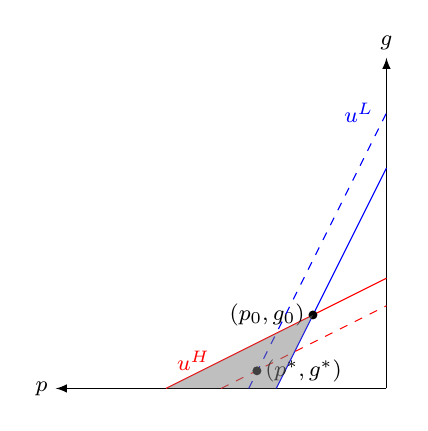
\begin{tikzpicture}[scale=0.7]
          \footnotesize
          % Axes: p is reversed and g is normal
          \draw[->, >=latex] (6,0) -- (0,0) node[left] {\( p \)}; % Reverse the p-axis
          \draw[->, >=latex] (6,0) -- (6,6) node[above] {\( g \)};
      
          % add text on (3,1), u^H in red color
          \node[red] at (2.5,0.5) {\( u^H \)};
          % add text on (3,5), u^L in blue color
          \node[blue] at (5.5,5) {\( u^L \)};
      
          % add lines 
          \draw[red] (2,0) -- (6,2);
          \draw[blue] (4,0) -- (6,4);
      
          % plot the intersection point 
          \filldraw[black] (14/3,4/3) circle (2pt) node[left] {\((p_0, g_0)\)};
      
          % add dashed lines
          \draw[dashed, red] (3,0) -- (6,3/2);
          \draw[dashed, blue] (3.5,0) -- (6,5);
          \filldraw[black] (3.65,0.32) circle (2pt) node[right] {\((p^*, g^*)\)};
        
          % shadow the area of (2, 0) -- (4, 0) -- (14/3, 4/3)
          \fill[gray, opacity=0.5] (2,0) -- (4,0) -- (14/3, 4/3) -- cycle;
        \end{tikzpicture}
        \caption{\footnotesize
          Indifference Curves with Reversed \( p \) axis}
        \label{fig:indifference_curves}
      \end{figure}
    \end{column}
    \begin{column}{0.5\textwidth}
      
      Given outside option \((p_0, g_0)\), firm designs plan \((p^*, g^*)\) to ensure self-selection:
      \[
      \left\{
      \begin{aligned}
      \alpha p^* + \beta^L g^* &> \alpha p_0 + \beta^L g_0, \\
      \alpha p^* + \beta^H g^* &< \alpha p_0 + \beta^H g_0,
      \end{aligned}
      \right.
      \]
      $$ \Rightarrow p^* < p_0, \quad g^* < g_0. $$

      Results:
      \begin{itemize}\small
        \item Low spenders prefer inside option $(p^*, g^*)$
        \item High spenders prefer outside option $(p_0, g_0)$
        \item Firm maximizes profit by offering $(p^*, g^*)$ to attract low spenders.
      \end{itemize}
    \end{column}
  \end{columns}
\end{frame}

\begin{frame}{Research Questions}
  \begin{itemize}
    \item How do MA firms strategically design plans to leverage private health perceptions and encourage self-selection among Medicare beneficiaries?
    \item What are the welfare implications of such strategic behavior?
  \end{itemize}
  
\end{frame}


\section{Empirical Model}

\begin{frame}{Timing}
  \begin{itemize}
    \item \textbf{Government Sets Capitation:} Determines capitation payments based on observable individual characteristics.
    \item \textbf{Stage 1 - Firm Decision:} Given plan offerings, Firms set the price and generosity levels of their plans to optimize profit after captiation.
    \item \textbf{Stage 2 - Consumer Choice:} Consumers select plans (including outside option) that best suit their own needs, leveraging their own private information.
  \end{itemize}
\end{frame}

\begin{frame}{Demand: Private Information}
  Each consumer is characterized by two variables:
  \begin{itemize}
      \item observable risk-adjusted capitation rate ($k_i$), which serves as a proxy for the average expected health expenditure within a similar health cohort.
      \item unobservable health perception ($e_i$), which directly influences their preference on plan generosity, and hence their plan choice.
  \end{itemize}

  \begin{equation}
    \ln(e_i) = \ln(k_i) + \tau_i, \quad \tau_i \sim N(0, \sigma_\tau^2)
  \end{equation}

\end{frame}

\begin{frame}{Demand: Utility}

  The utility of consumer $i$ from plan $j$ is given by

  \begin{equation}
    u_{ij} = \beta_i g_j - \alpha_i p_j + \lambda^{A}_i A_j + \lambda^X X_j + \xi_j + \varepsilon_{ij}.
  \end{equation}

  \begin{itemize}\small
    \item $g_j$ and $p_j$ are the generosity and premium of plan $j$.
    \item $A_j$ is MA type indicator
    \item $X_j$ is a vector of other plan characteristics
    \item $\xi_j$ is the unobserved plan-specific quality
    \item $\varepsilon_{ij}$ is the idiosyncratic error term, following a T1EV distribution
  \end{itemize}

  The utilitiy of the outside option (TM + Medigap) is
  \begin{equation}
    u_{i0} = \beta_i g_0 - \alpha_i p_0 + \xi_0 + \varepsilon_{i0}.
  \end{equation}
\end{frame}

\begin{frame}{Demand: Hetereogeneity}

  Preferences for plan generosity ($\beta_i$) are influenced by health perception $e_i$
  \begin{equation}
      \beta_i = \bar{\beta} + \gamma \ln e_i.
  \end{equation}
  Preferences for plan premiums ($\alpha_i$) are associated with income level
  \begin{equation}
      \alpha_i = \bar{\alpha} + \rho^{\text{inc}} \text{inc}_i.
  \end{equation}
  Preferences for the MA type ($\lambda^{A}_i$) relate to demographic factors and existing health coverage, including Medicaid eligibility and employer-sponsored insurance (ESI) coverage
  \begin{equation}
      \lambda^{A}_i = \bar{\lambda}^{A} + \rho^{\text{edu}} \text{edu}_i + \rho^{\text{white}} \text{white}_i + \rho^{\text{Mcd}} \text{Mcd}_i + \rho^{\text{ESI}} \text{ESI}_i.
  \end{equation}
  
\end{frame}

\begin{frame}{Demand: Plan Mean Utility}
  The mean utility of plan $j$ relative to the outside option is

  \begin{equation}
    \delta_j = \bar{\beta} (g_j - g_0) - \bar{\alpha} (p_j - p_0) + \bar{\lambda}^{A} A_j + \lambda^X X_j + \xi_j - \xi_0,
  \end{equation}
  and let the $\mu_ij$ denote the individual-specific deviation from $\delta_j$, we can rewrite the utility function as
  \begin{equation}
    u_{ij} = \delta_j + \mu_{ij} + \varepsilon_{ij}.
  \end{equation}

\end{frame}

  

\begin{frame}{Demand: Plan Choice Probability}
  Considering the T1EV distribution of $\varepsilon_{ij}$, the probability that consumer $i$ chooses plan $j$ is given by
  \begin{equation}
    s_{ij}(e_i) = 
    \frac{\exp \big(\delta_j + \mu_{ij}(e_i) \big)}
    {\sum_{j' = 0}^{J}  \exp \big(\delta_{j'} + \mu_{ij'}(e_i) \big)}.
  \end{equation}

  The market share of plan $j$ is given by the weighted sum of the individual choice probabilities
  \begin{equation}
    q_j = \sum_i w_i \cdot s_{ij}(e_i) = \sum_i w_i \cdot \int s_{ij}(e) \, dF_{e}(e).
\end{equation}
\begin{itemize}\small
  \item $w_i$ is the sampling weight of consumer $i$
\end{itemize}

\end{frame}

\begin{frame}{Supply: Competition Setting}
  \begin{itemize}
    \item \textbf{Bertrand-Nash}: Firms compete in prices and plan generosity levels, given plan offerings and other exogenous attributes, with each plan having its specific cost functions.
    \item \textbf{Multi-Product Multi-Market}: Firms operate as multi-product entities competing across multiple submarkets.
    \item \textbf{Focus on Short Run}: The model does not account for the entry and exit of plans.
  \end{itemize}
\end{frame}

\begin{frame}{Supply: Costs}

  This cost is influenced by the plan's generosity level $g_j$ and other observable exogenous attributes $X_j$. The marginal cost function is expressed as
  \begin{equation}
    \label{eq:marginal_cost}
    mc_j(g_j) = mc_j^g(g_j) + \underbrace{w^X \cdot X_j + \omega_j}_{\text{predetermined}},
  \end{equation}
  \begin{itemize}\small
    \item unobserved plan-specific cost shock $\omega_j$,
    \item each plan has a unique cost function due to the perdetermined components.
  \end{itemize}


\end{frame}

\begin{frame}{Supply: Profits}
  The profit function for plan $j$ in county $c$, which has a market size of $M_c$, is
  \begin{equation}
      \pi_j = (b_j - mc_j(g_j)) \cdot M_c \cdot s_{c,j}(g, b).
  \end{equation}

  \begin{itemize}\small
    \item Supplementary Bid  $b_j$: Price received by the firm.
    \item Premium $p_j$:  Price paid by the consumer.
    \item Premium Reduction $p^\text{reduc}$: Difference, assumed to be exogenous and fixed.
    \item Premium Calculation: \( p_j = b_j - p^\text{reduc} \), linking  bid to premium.
  \end{itemize}

\end{frame}


\begin{frame}{Supply: Plan Design Problem}
  The total profit for a firm in county $c$ is the aggregate of profits from all its offered plans
  \begin{equation}
      \pi_{f,c} = \sum_{j \in \mathcal{J}_{f,c}} \pi_{j}.
  \end{equation}

  The state-level profit for MA firm $f$ is then the sum of profits across all counties $c$ where firm $f$ operates
  \begin{equation}
      \pi_{f} = \sum_{c \in \mathcal{C}_f} \pi_{f,c},
  \end{equation}
  where $\mathcal{C}_f$ denotes the set of counties in which firm $f$ is active.

  The firm's plan design problem can be formulated as maximizing state-level profit by strategically setting bid and generosity levels for each plan
  \begin{equation}
  \label{eq:objective_function}
      \max_{b_f, g_f} \pi_{f} = \sum_{c \in \mathcal{C}_f } \sum_{j \in \mathcal{J}_{f,c} } (b_j - mc_j(g_j)) \cdot M_c \cdot s_{c,j}(g, b),
  \end{equation}

\end{frame}

\begin{frame}{Supply: Necessary Optimality Conditions}
  The first-order conditions for the firm's plan design problem are
  \begin{equation}
    \label{eq:bid_foc}
        \{b_j\}: \quad \sum_{c \in \mathcal{C}_f} 
        M_c \left(s_{c,j} + \sum_{j \in \mathcal{J}_{f,c}} (b_j - mc_j) \cdot \frac{\partial s_{c,j}}{\partial b_j} \cdot
        \frac{\partial b_j}{\partial p_j} \right) = 0 
        \quad \forall j,
    \end{equation}
    \begin{equation}
    \label{eq:generosity_foc}
        \{g_j\}: \quad \sum_{c \in \mathcal{C}_f} 
        M_c \left( 
            \frac{\partial mc_j}{\partial g_j} \cdot s_{c,j} - 
            \sum_{j \in \mathcal{J}_{f,c}}
            (b_j - mc_j) \cdot \frac{\partial s_{c,j}}{\partial g_j}
        \right) = 0
        \quad \forall j,
    \end{equation}
    where $\frac{\partial b_j}{\partial p_j} = 1$.

    Each firm faces unique optimization conditions due to differences in plan offerings and the specifics of their cost functions (see Equation \ref{eq:marginal_cost}).

\end{frame}

\section{Estimation}

\begin{frame}{Estimation: Demand Overview}
  Two step estimation by \citet{goolsbeeConsumerGainsDirect2004}

  \begin{itemize}
    \item Weighted MLE of the heterogeneity parameters and mean utilities.
    \item IV estimation of the mean utility parameters.
  \end{itemize}
\end{frame}

\begin{frame}{Weighted MLE}
  Find $\vartheta$ that maximizes the likelihood of the observed individual choices, while ensuring that the implied market shares match the observed market shares.

  \begin{equation}
    \begin{aligned}
        \max_\vartheta
                            & \underbrace{\sum_{c} \sum_i w_{ci} \cdot \sum_{j\in \mathcal{J}_c}
            y_{cij} \cdot \ln(s_{cij} (\vartheta ))}
        _{\text{Weighted log-likelihood}}                                                        \\
        \textrm{s.t.} \quad & \underbrace{{s_{cj}^*} =
            \sum_i w_{ci} \cdot s_{cij} (\vartheta )}_{\text{Market share matching condition}}
        \quad \forall j = 1, ...J, \quad \forall c,                                              \\
    \end{aligned}
\end{equation}
\begin{itemize}\small
  \item $y_{cij}$ is the indicator of the observed individual choice of plan $j$ in county $c$,
  \item $s_{cij}^*$ is the observed market share of plan $j$ in county $c$.
\end{itemize}
  
\end{frame}

\begin{frame}{Estimation: Consumer Heterogeneity}
  
\begin{table}[ht]\footnotesize
    \centering
    \caption{Estimation Results of Consumer Preference Heterogeneity}
    \label{tab:demand_result_1}
    \begin{tabular}{lccc}
        \toprule
        \textbf{Variable} & \textbf{Parameter} & \textbf{Estimate} & \textbf{Std Error} \\
        \midrule
        \textbf{Generosity Preference} & & & \\
        Health Perception & $\gamma$ & 0.115 & (0.052) \\
        \midrule
        \textbf{Premium Preference} & & & \\
        High Income Level & $\rho^{\text{inc}}$ & -0.473 & (0.248) \\
        \midrule
        \textbf{MA Type Preference} & & & \\
        High Education Level & $\rho^{\text{edu}}$ & -0.275 & (0.203) \\
        White Race & $\rho^{\text{white}}$ & -0.173 & (0.280) \\
        Medicaid Coverage & $\rho^{\text{Mcd}}$ & 0.039 & (0.244) \\
        ESI Coverage & $\rho^{\text{ESI}}$ & -2.543 & (0.404) \\
        \midrule
        \textbf{Private Information Distribution} & & & \\
        SD of Health Perception & $\sigma_{\tau}$ & 3.983 & (2.733) \\
        \bottomrule
    \end{tabular}
    \begin{threeparttable}
        \begin{tablenotes}\footnotesize
            \item \textit{Note}: ESI stands for employer-sponsored insurance.
        \end{tablenotes}
    \end{threeparttable}
\end{table}

\end{frame}


\begin{frame}{IV}
  \begin{columns}
    \begin{column}{0.5\textwidth}
      \begin{figure}[htbp]
        \centering
        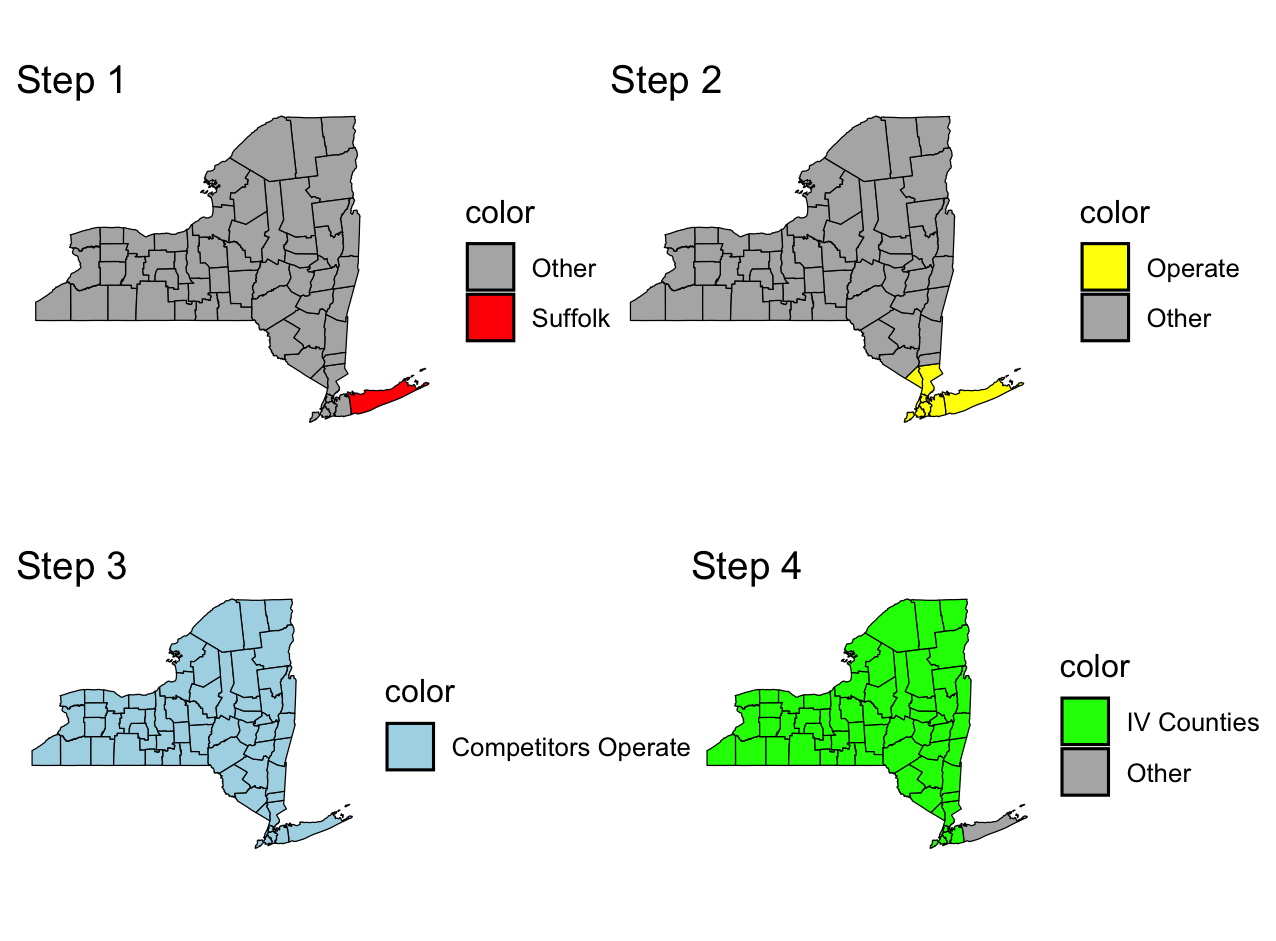
\includegraphics[width=1\textwidth]{figures/images/iv_map.png}
        \caption{IV Construction Process}
        \label{fig:IV_construction}
      \end{figure}

    \end{column}

    \begin{column}{0.5\textwidth}
      Based on methodology from \citet{fanOwnershipConsolidationProduct2013}.
      \begin{itemize}\small
          \item \textbf{IV Construction Rationale:} Utilizes demographics from markets where the plan does not operate but its overlapping competitors do.
          \item \textbf{Key Insight:} Demographics in non-operating markets influence competitor actions, only indirectly affecting the plan of interest through competition in plan design.
      \end{itemize}
      
    \end{column}
      
    
  \end{columns}
  
\end{frame}


\begin{frame}{Plan Mean Utility}
  \begin{table}[htbp]\footnotesize
  % add title and caption
  \caption{Estimation Results of Plan Mean Utility}
  \label{tab:demand_result_2}
  \centering
  \begin{tabular}{lccc}
  \toprule
  \textbf{Variable} & \textbf{Parameter} & \textbf{Estimate} & \textbf{Std Error} \\
  \midrule
  \textbf{Coverage} & & & \\
  MA Type & $\bar{\lambda}^{A}$ & -1.917 & (0.224) \\
  Premium & $\bar{\alpha}$ & -1.316 & (0.354) \\
  Generosity & $\bar{\beta}$ & 1.006 & (0.388) \\
  \midrule
  \textbf{Network} & & \\
  Rating (per star) & -  & 0.282 & (0.028) \\
  HMO & - & 0.204 & (0.029) \\
  \midrule
  \textbf{Additional Benefits} & & &\\
  Dental  & - & -0.077 & (0.033) \\
  Vision  & - & -0.015 & (0.031) \\
  Hearing  & - & 0.031 & (0.034) \\
  \bottomrule
  \end{tabular}
\end{table}
\end{frame}


\begin{frame}{Estimation: Supply Overview}
  \begin{itemize}
      \item Estimation builds on first-order conditions from supply model, integrating estimated consumer response from demand side.
      \item Similar to demand side, supply side estimation faces issues due to unobservable factors correlating with plan design variables.
      \item Utilizes the same IV strategy as in demand estimation to address endogeneity.
  \end{itemize}
\end{frame}

\begin{frame}{Plan Costs}
  \begin{table}[ht]\scriptsize
    \centering
    \begin{threeparttable}
        \caption{Estimation of Plan Marginal Cost}
        \begin{tabular}{lcccc}
        \toprule
        & \multicolumn{2}{c}{\textbf{I}} & \multicolumn{2}{c}{\textbf{II}} \\
        \multirow{1}{*}{\textbf{Variable}} & \textbf{Estimate} & \textbf{Std Error} & \textbf{Estimate} & \textbf{Std Error} \\
        \midrule
        \textbf{Coverage} & & & & \\
        Generosity & 1.353 & (0.171) & 1.367 & (0.174) \\
        $\text{Generosity}^2$ & 0.160 & (0.020) & 0.140 & (0.021) \\
        \midrule
        \textbf{Network} & & & & \\
        Rating (per star) & 0.150 & (0.019) & 0.157 & (0.020) \\
        HMO & 0.237 & (0.022) & 0.247 & (0.023) \\
        \midrule
        \textbf{Additional Benefits} & & & & \\
        Dental  & 0.170 & (0.023) & 0.158 & (0.025) \\
        Vision  & 0.039 & (0.055) & 0.045 & (0.055) \\
        Hearing  & 0.095 & (0.026) & 0.118 & (0.027) \\
        \midrule
        \textbf{Firm Fixed Effect} & & & & \\
        Aetna & - & - & -0.017 & (0.033) \\
        Anthem & - & - & -0.181 & (0.049) \\
        UHG & - & - & -0.079 & (0.030) \\
        \bottomrule
        \end{tabular}
        % \begin{tablenotes}
        %     \item \textit{Note}: Estimation I is without firm fixed effects, II is with firm fixed effects.
        % \end{tablenotes}
    \end{threeparttable}
\end{table}
\end{frame}

\begin{frame}{Summary by Plan Generosity Choices}
  \begin{table}[ht]
    \centering
    \caption{Summary of Plan Costs by Generosity Quartile}
    \label{tab:result_summary_g}
    \begin{threeparttable}
    \begin{tabular}{@{}lccccc@{}}
    \toprule
    \textbf{Generosity Quartile}  & \textbf{Cost} & \textbf{Capitation} & \textbf{$\text{Capitation}-\text{Cost}$} & \textbf{Bid}   \\ \midrule
    1st Quartile (Lowest)    & 9.136    & 9.560      & 0.424   & 0.556         \\
    2nd Quartile             & 9.629    & 9.931      & 0.305   & 0.701         \\
    3rd Quartile             & 10.364   & 10.495     & 0.134   & 0.900         \\
    4th Quartile (Highest)   & 12.516   & 12.168     & -0.348    & 1.417         \\ \bottomrule
    \end{tabular}
    \footnotesize
    \begin{tablenotes}
        \item \textit{Note}: Values are in thousand dollars. The capitation represents the subsidy received by MA firms from CMS. Bid refers to the supplemental bid that supposed to cover the cost of additional benefits. The difference between capitation and cost is the profit margin of the plan without bid.
    \end{tablenotes}
    \end{threeparttable}
    \end{table}
\end{frame}

\begin{frame}{Summary by Plan Generosity Choices}
  \begin{figure}[htbp]
    \centering
    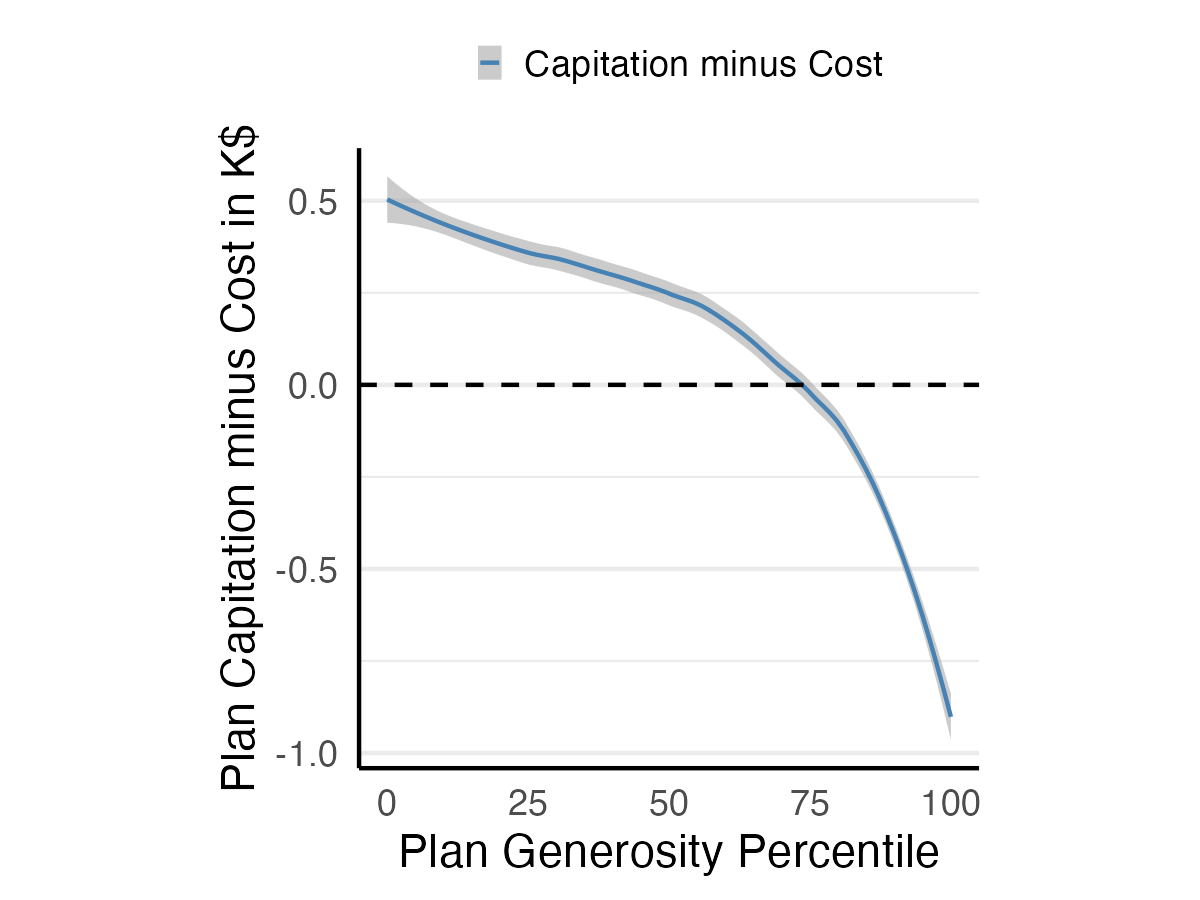
\includegraphics[width=0.5\textwidth]{figures/images/profit_without_premium_kernal.png}
    \caption{Capitation minus Cost by Plan Generosity Percentile}
    \label{fig:profit_without_premium_kernal}
    % add vertical space
    \vspace{0.1cm}
    \begin{minipage}{0.8\textwidth}
        \footnotesize
        \textit{Note}: The 95\% confidence interval is depicted in the plot.
    \end{minipage}
\end{figure}
\end{frame}



\section{Welfare Outcome}

\begin{frame}{Welfare Analysis}
  \begin{table}
    \centering
    \caption{Summary of Current Market}
    \begin{tabular}{|l|c|c|}
    \hline
    \textbf{Category}                            & \textbf{Per Capita} & \textbf{National Total}  \\ \hline
    Consumer Surplus                             & \$382               & \$22.08 billion          \\ \hline
    Producer Surplus                             & \$1,068             & \$14.45 billion          \\ \hline
    Gov Spending on TM                           &  -                   & \$370.26 billion         \\ \hline
    Gov Spending on MA                           &  -                   & \$163.51 billion         \\ \hline
    Total Gov Spending                           &  -                   & \$533.77 billion         \\ \hline
    \end{tabular}
  \end{table}
\end{frame}

\begin{frame}{Future Work}
  Counterfactual Simulation
  \begin{itemize}
    \item \textbf{Simulate Equal-Profit}: profit only depends on quantities, not the type of enrollees. No gaming incentives for firms.
    \item \textbf{Quantify Selection Effect}: the welfare difference between the observed and counterfactual market outcome.
  \end{itemize}
\end{frame}

%---- The ending ----%
\begin{frame}[plain, noframenumbering] % Create a new frame without a frame number
  \begin{center}
  \Huge \textit{Thank You!} % Use a huge font size for the text "Thank You!"
  \end{center}
\end{frame}

%---- Bibliography ----%
\newpage
\begin{frame}[plain, noframenumbering] % Create a new frame without a frame number
  \frametitle{References} % Add a title to the slide

  \bibliographystyle{aer} % set the bibliography style as AER
  \bibliography{bibliography} % set the bibliography file (bibliography.bib)
\end{frame}

%---- The appendix ----%
\appendix
\begin{frame}[plain, noframenumbering] % Create a new frame without a frame number
  % show the title of the appendix centered on the slide
  \begin{center}
    \Huge Appendix
  \end{center}
\end{frame}

\begin{frame}{Appendix: Risk Adjustment Generation}
  \begin{figure}
    \centering
    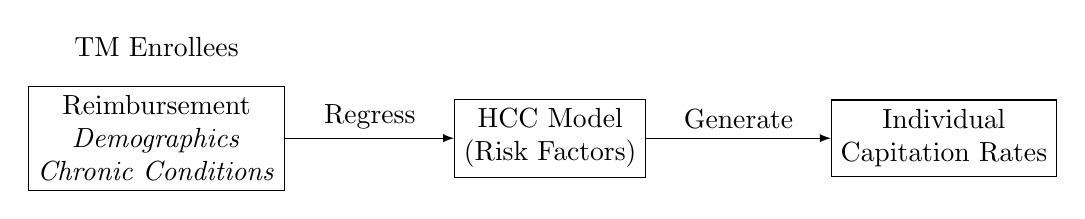
\begin{tikzpicture}
    \node[draw, rectangle, align=center] (input) at (0,0) { Reimbursement \\  \textit{Demographics}  \\  \textit{Chronic Conditions}};
    \node[above=0.25cm of input] {TM Enrollees};
    \node[draw, rectangle, align=center] (model) at (5,0) {HCC Model \\ (Risk Factors)};
    \node[draw, rectangle, align=center] (output) at (10,0) {Individual \\ Capitation Rates};
    
    \draw[->, >=latex] (input) -- (model) node[midway,above] {Regress};
    \draw[->, >=latex] (model) -- (output) node[midway,above] {Generate};
\end{tikzpicture}
    \caption{Capitation Rate Generation Process}
  \end{figure}
\end{frame}

\begin{frame}{Appendix: Risk Adjustment Outcomes}
  \begin{columns}
    \begin{column}{0.5\textwidth}
      \begin{figure}
        \centering
        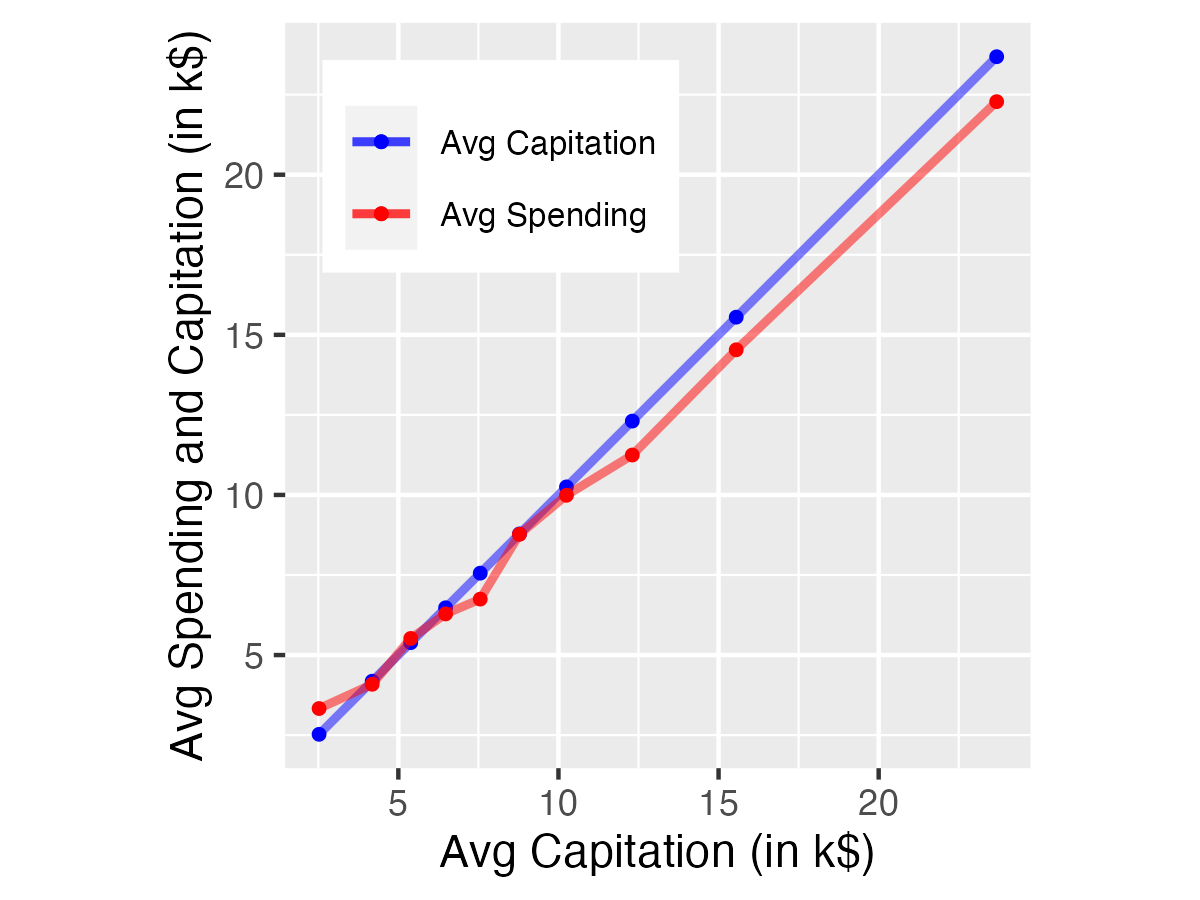
\includegraphics[width=1\textwidth]{figures/images/avg_spending_vs_capitation_by_capitation_deciles.png}
        \caption{Conditional on Capitation Deciles}
      \end{figure}
    \end{column}
    \begin{column}{0.5\textwidth}
      \begin{figure}
        \centering
        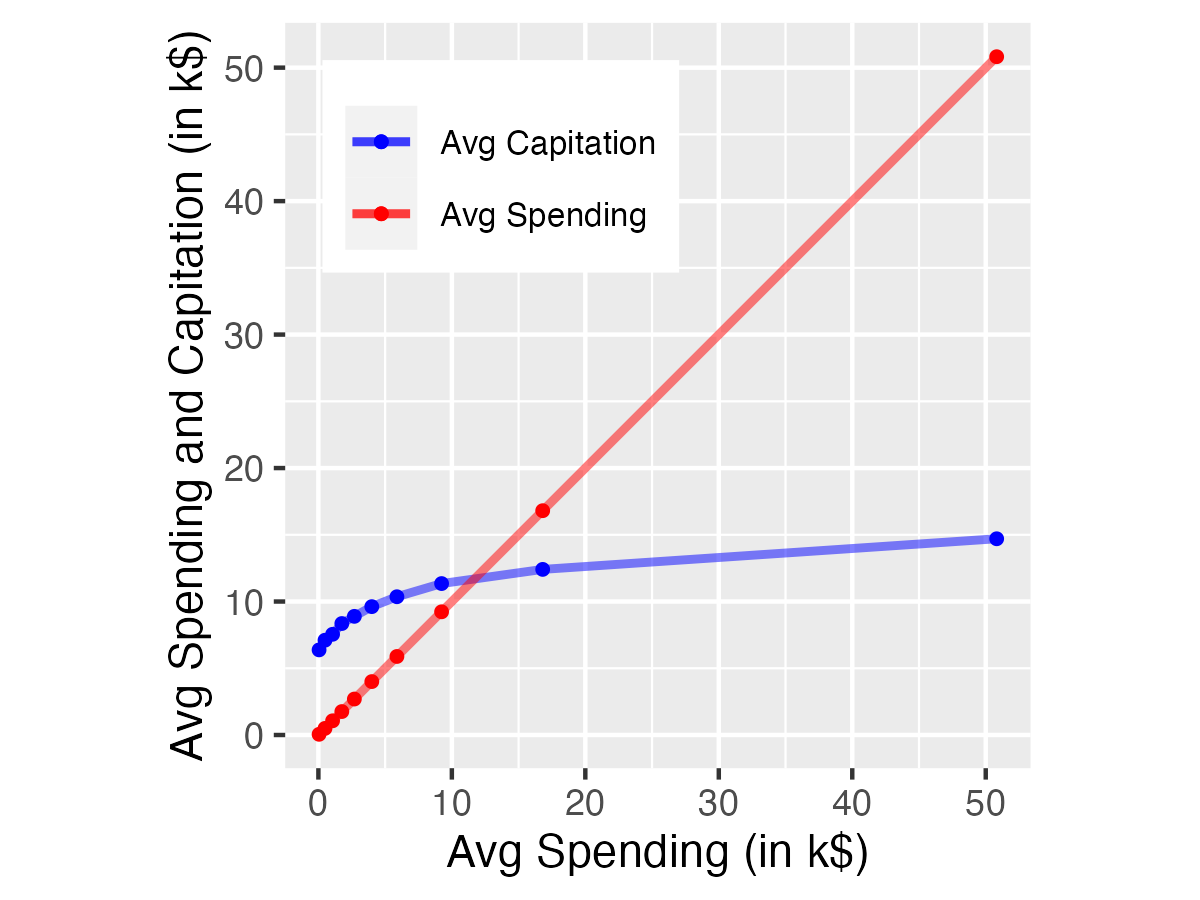
\includegraphics[width=1\textwidth]{figures/images/avg_spending_vs_capitation_by_spending_deciles.png}
        \caption{Conditional on Spending Deciles}
      \end{figure}
    \end{column}
    
  \end{columns}
\end{frame}

\begin{frame}{Appendix: Benefit Structure}
  \begin{figure}
    \begin{figure}
      \centering
      \resizebox{0.8\textwidth}{!}{\usetikzlibrary{positioning, fit, backgrounds}
\begin{tikzpicture}[
    block/.style={
      draw,
      rectangle,
      rounded corners,
      minimum height=2cm, 
      minimum width=3cm, 
      align=center
    },
    node distance=0.5cm
]
% Nodes of MA coverage
\node[block] (ma) {Medicare Basic\\Part A\&B Coverage};
\node[block, right=of ma] (supp) {MA\\Supplementary\\Part A\&B Coverage};
% make the add node in dashed line
\node[block, right=of supp, dashed] (add) {Additional Benefits \\ (e.g. Dental)};

% group the nodes
\begin{scope}[on background layer]
    % add title MA Benefits over the nodes
  \node[above=0.5cm of supp] {Medicare Advantage};
  \node[fit=(ma) (supp) (add), draw, inner sep=0.5cm] (ma_group) {};
\end{scope}

% add space between the two groups
\node[below=1cm of ma_group] {};

% Nodes of Medigap coverage
\node[block, below=2cm of ma] (medigap) {Medicare Basic\\Part A\&B Coverage};
\node[block, right=of medigap] (medigap_supp) {Medigap\\Supplementary\\Part A\&B Coverage};


% group the nodes
\begin{scope}[on background layer]
    % add title Medigap Benefits over the nodes
  \node[above=0.5cm of medigap_supp] {TM+Medigap};
  \node[fit=(medigap) (medigap_supp), draw, inner sep=0.5cm] (medigap_group) {};
\end{scope}

\end{tikzpicture}}
    \end{figure}
  \end{figure}
\end{frame}

\end{document}